\documentclass[compress,dvips,xcolor={dvipsnames},t]{beamer}

\usepackage[english]{babel}
\usepackage{graphicx}
\usepackage{amssymb,amsmath,amsthm}
\usepackage{xspace}
\usepackage{hyphenat}

\newtheorem{proposition}{Proposition}
%\newtheorem{theorem}{Theorem}
\newcommand{\id}[1]{\textsf{#1}}
\newcommand{\coding}[4]{#1 \vdash #2 : #3 \rightarrow #4}
\newcommand{\decoding}[3]{{\cal D}(#1,#2,#3)}

\renewcommand{\refname}{}
\newcommand\ASN{\textsf{ASN.1}\xspace}
\newcommand{\core}{core \ASN}
\newcommand\Cpp{\mbox{\textsf{C} \hspace*{-2.5mm} \raise 0.7mm \hbox
{${\scriptscriptstyle \textsf{++}}$}}\xspace}

\title{Career overview}
\author{Christian Rinderknecht}
\date{20 May 2026}

\begin{document}

\frame{\maketitle}


\begin{frame}
  \frametitle{A personal introduction}

  \begin{itemize}

    \item My alma mater is \emph{Universit\'e Pierre et Marie Curie}
      (UPMC, a.k.a. Paris~6).

    \item I did my doctoral studies at Inria, one of the most
      prestigious research institutes in informatics in France.

    \item I was a member of the team that developed the programming
      language OCaml. I am still in touch with the team.

    \item I went on to work as an engineer, a researcher and a
      professor for many years, across several countries (France,
      Korea, Hungary, Sweden), both in academia and private
      companies.

    \item My main expertise domains are the design of programing
      languages, compiler construction, functional programming and
      didactics of programming languages.

  \end{itemize}

\end{frame}

%%%%%%%%%%%%%%%%%%%

\begin{frame}
  \frametitle{A personal introduction}

  \begin{minipage}{0.5\linewidth}
    My book about functional programming and the analysis of
    algorithms is published by King's College London (600 pages).
  \end{minipage}%
  \begin{minipage}{0.5\linewidth}
    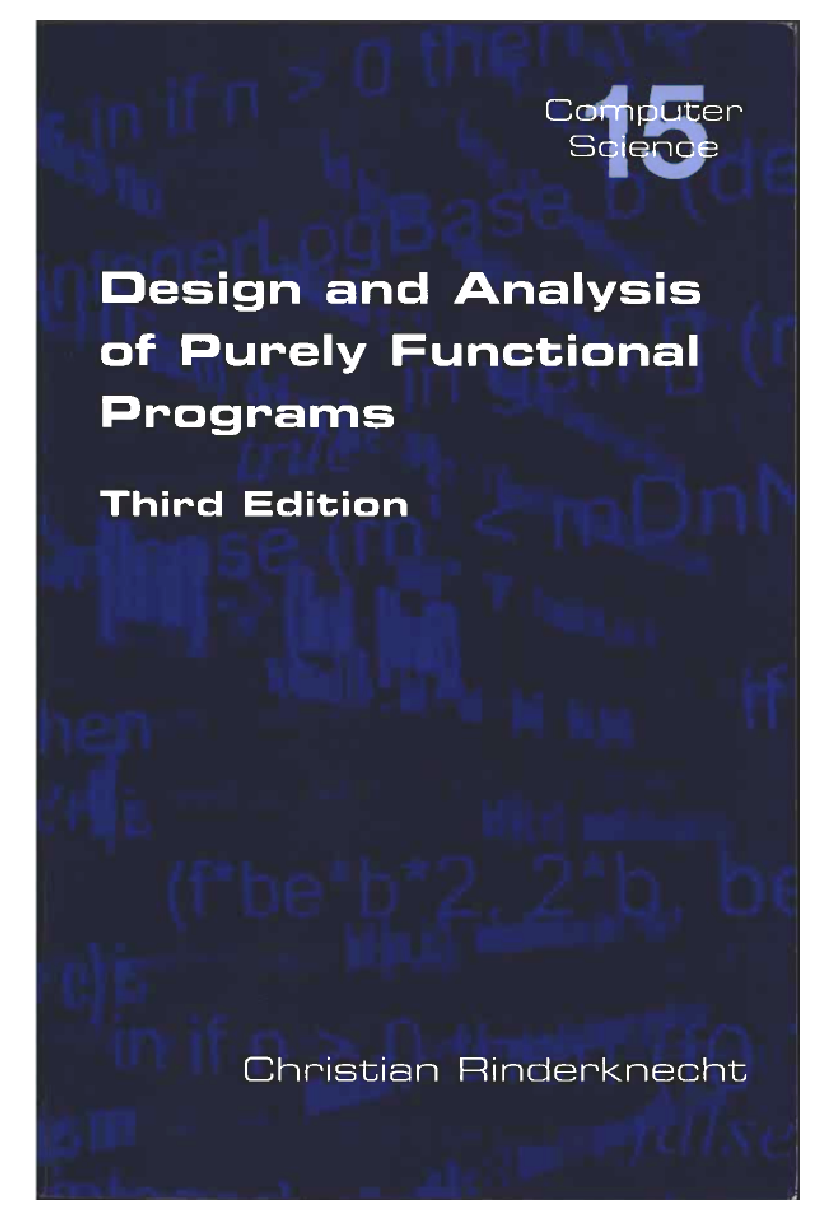
\includegraphics[scale=0.35]{my_book.eps}
  \end{minipage}%

\end{frame}

%%%%%%%%%%%%%%%%%%%

\begin{frame}
  \frametitle{Career}

  I propose a simplified thematic approach:
  \begin{enumerate}

    \item the design of programming languages and their compilation
      (front\hyp{}ends, type\hyp{}checkers, static analysis);

    \item the didactics of programming languages and the analysis of
      algorithms;

    \item the teaching of programming languages and their models.

  \end{enumerate}

  \bigskip

  My work on compiler construction is split between academia and
  industry, as 2/3 of my career was in academia.

  \bigskip

  I will hightlight only a few topics.

\end{frame}

%%%%%%%%%%%%%%%%%%%

\begin{frame}
\frametitle{Compiler front-ends -- The case of \ASN}

My doctoral studies were dedicated to applying formal logic from the
theory of programming languages to an industrial language in use in
telecommunications.

\medskip

The wide variety of hardware architectures and programming languages
calls for the definition of a universal format for data to be
exchanged over a computer network. \emph{Abstract Syntax Notation One}
(\ASN) is a standardised language (ISO, ITU-T) for defining data types
whose values may be exchanged across a network between two, possibly
heterogeneous peers.

\medskip

\ASN is completed by a set of \emph{encodings} which serialise the
values into streams of bits, the two most prominent being
\begin{itemize}

  \item the Basic Encoding Rules (BER),
  \item and Packed Encoding Rules (PER).

\end{itemize}

\end{frame}

%%%%%%%%%%%%%%%%%%%

\begin{frame}
\frametitle{Application domains of \ASN}

\begin{itemize}

  \item Telecommunication Management Network (SNMP, CMIP);

  \item Lightweight Directory Access Protocol (LDAP);

  \item email (\textsf{X.400});

  \item \textsf{UMTS} (Radio Access Network);

  \item Transferred Account Procedure~3 (billing for
    \textsf{GSM/UMTS} roaming);

  \item \textsf{3GPP LTE} (Long Term Evolution of \textsf{GSM/UMTS}
    networks);

  \item Multimedia conferencing systems with \textsf{H.323} (for
    signalling: \textsf{H.225}, \textsf{H.235}, \textsf{H.245},
    \textsf{H.248}, \textsf{H.450.1});

  \item Interactive television services (\textsf{MHEG});

\end{itemize}

\end{frame}

%%%%%%%%%%%%%%%%%%%

\begin{frame}
\frametitle{\ASN (usages, continued)}

\begin{itemize}

  \item Intelligent Transportation Systems (traffic signal
  control, electronic toll collection, emergency response etc.);

  \item Radio Frequency Identification (RFID);

  \item Aeronautical Telecommunication Network (air traffic control,
    flight information services, passenger communications, air-ground
    protocols etc.);

  \item Cryptography for electronic commerce over the internet (SET,
    PKCS~7, OpenSSL);

  \item Smart cards (SIM, WIM and VITALE);

  \item National Center for Biotechnology Information (NCBI):
    specification of millions of DNA sequences;

\end{itemize}

\end{frame}

%%%%%%%%%%%%%%%%%%%

\begin{frame}
\frametitle{\ASN (usages, continued)}

  \begin{itemize}

  \item client-server protocol for database access (U.S. Library of
    Congress: \textsf{Z39.50});

  \item \ASN is embedded in other specification and programming
    languages like System Design Language (SDL, control), Message
    Sequence Charts (MSC, functional requirements), Testing and Test
    Control Notation (TTCN-3, tests suites), etc.

  \item \ASN is also used without formal control specification by
    protocol designers and tool implementors, \emph{e.g.}, SNMP,
    OpenSSL.

\end{itemize}

\end{frame}

%%%%%%%%%%%%%%%%%%%

\begin{frame}
\frametitle{\ASN and the compilation chain}

\begin{center}

\includegraphics[scale=0.5]{compilation.eps}
\end{center}

\end{frame}

\begin{frame}
\frametitle{How do \ASN and the BER interact?}

\begin{itemize}

  \item Both peers share a common \ASN specification and agree upon
    the usage of the BER;

  \item each peer compile the \ASN specification to a set of type
    declarations and a set of coders/decoders (codecs) for each type;

  \item the target language may be different depending on the peer;

  \item the coders transform a value into a stream of bits according
    to the BER,

  \item the decoders transform a stream of bits into a value according
    to the BER (or reject it as ill-formed);

  \item these pieces of source code are compiled and linked separately
    against the corresponding communicating applications.

\end{itemize}

\end{frame}

%%%%%%%%%%%%%%%%%%%

\begin{frame}
\frametitle{General issues}

\begin{enumerate}

  \item Specifications: huge (700 pages A4, 10pt), complex (concepts
    mutually dependent).

  \item Syntax: large and ambiguous grammar, dynamic extensions.

  \item English cannot tell the meaning of all combinations of
    syntactical constructs.

  \item Types denote value sets and type operators denote set
    operations: subtypes yield general set constraints.

  \item Encoding only applies to a subset of \ASN, defined
    implicitly and dependent on the encoding rules.

  \item Decoding is unspecified.

  \item Dynamic checks in codecs (depending on the target programming
    language) are unspecified.

  \item Open source or free compilers: extremely rare, unmaintaned,
    fragile, without precise error reporting.

\end{enumerate}

\end{frame}

%%%%%%%%%%%%%%%%%%%

\begin{frame}
\frametitle{Syntax analysis}

The BNF of \ASN is larger than that of ISO \Cpp.

\bigskip

When fed to Yacc as it is specified in the standards, it yields
between 3,000 and 4,000 shift/reduce and reduce/reduce conflicts
(for each kind!). Unsurprisingly, it is ambiguous.

\bigskip

The situation is actually much worse: many \emph{tokens} are
ambiguous, so if the lexer works without any extra knowledge from the
parser, there are even more conflicts.

\bigskip

I first solved the problem of the syntax analysis on the 1990
standard, which is smaller, albeit very nasty as well.

\end{frame}

%%%%%%%%%%%%%%%%%%%

\begin{frame}
\frametitle{Theoretical Problems}

\begin{enumerate}

  \item \label{finiteness} the types may have only infinite
        values:\\
        \texttt{T ::= SET \{a T\}};

  \item \label{type_conformance} some value declarations may be
        ill-typed:\\
        \texttt{v REAL ::= ""};

  \item \label{type_compatibility} especially, some value references
        may be ill-typed, as\\
        \texttt{a VisibleString ::= b}\\
        \texttt{b INTEGER ::= 0};

  \item \label{constraint_consistence} the subtype constraints may
        be inconsistent:\\
        \texttt{T ::= REAL (SIZE(7))};

  \item \label{subtype_non_emptiness} the subtypes may be empty, as\\
        \texttt{T ::= SET ((SIZE (1)) \symbol{94} (SIZE (2))) OF REAL};

  \item \label{solvability} the subtypes may have no value set:\\
        \texttt{T ::= REAL (ALL EXCEPT T)}.

\end{enumerate}

\end{frame}

%%%%%%%%%%%%%%%%%%%

\begin{frame}
\frametitle{Problems (cont.)}

In other words, the issues to settle are respectively:
\begin{enumerate}

  \item the finiteness problem;

  \item the typechecking problem;

  \item the type compatibility problem;

  \item the constraint consistence problem;

  \item the non-emptiness problem;

  \item the solvability problem.

\end{enumerate}

\medskip

I showed that finiteness and solvability are enough to get a full
validation of \ASN.

\medskip

I designed an algorithm to extract set constraints from \ASN
specifications.

\end{frame}

%% \begin{frame}
%% \frametitle{Analysis}

%% \begin{itemize}

%%   \item type compatibility $\subseteq$ typechecking;

%%   \item constraint consistence, non-emptiness $\subseteq$ solvability
%%         (the system is solved when we construct explicitly the values
%%         of each subtype);

%%   \item typechecking $\subseteq$ solvability:
%% \begin{tabular}{@{}r@{\,}c@{\,}l@{}}
%%    \texttt{y INTEGER (0..9) ::= 1}
%%    & $\rightarrow$
%%    & $\left\{
%%        \begin{tabular}{@{\,}l@{}}
%%            \texttt{y A ::= 1} \\
%%            \texttt{A ::= INTEGER (0..9)} \\
%%            \texttt{B ::= A (y)}
%%         \end{tabular}
%%      \right.$
%% \end{tabular}
%% where \texttt{A}~and~\texttt{B} are fresh type references.

%% \end{itemize}

%% So, finiteness and solvability are enough to get a full validation of
%% \ASN.

%% \end{frame}

%%%%%%%%%%%%%%%%%%%

%% \begin{frame}
%% \frametitle{Set Constraints}

%% Sets constraints are inclusions between expressions interpreted over
%% the domain of sets of trees which may be recursively defined.

%% \medskip

%% The \ASN types, by having a tree structure (technically, they are
%% rational trees), fit perfectly in the usual domain of set
%% constraints.

%% \medskip

%% A set constraint has the form $\alpha \subseteq \beta$, where $\alpha$
%% and $\beta$ are \emph{set expressions}. Examples are \textsf{0} (the
%% empty set), \textsf{1} (the set of all terms), $\alpha$ (a set-valued
%% variable), $c(\alpha, \beta)$ (a constructor application), and the
%% union, intersection or complement of set expressions. Given a set of
%% constructors ${\cal C}$, where each $c \in \mathcal{C}$ has arity
%% $a(c)$, set expressions are defined by the grammar:
%% \begin{equation*}
%% E ::= \textsf{0} \mid \textsf{1} \mid \alpha \mid c (E_1, \ldots,
%% E_{a(c)}) \mid E_1 \cup E_2 \mid E_1 \cap E_2 \mid \neg E_1.
%% \end{equation*}

%% \end{frame}

%% %%%%%%%%%%%%%%%%%%%

%% \begin{frame}
%% \frametitle{Common Application}

%% In general, set constraints are used in the static analysis of
%% programs: they are the smallest supersets of the sets of the computed
%% values. Solving these constraints means constructing these
%% approximated sets (\emph{e.g.}, for optimisation).

%% \medskip

%% For example, consider a program with two uses of a variable
%% $v$. Assume that from one use we determine that $v$ must be a number
%% (\emph{i.e.}, $v \subseteq \textsf{Int} \, \cup \, \textsf{Float}$)
%% and from the other use that $v$ cannot be an integer (\emph{i.e.}, $v
%% \subseteq \neg\textsf{Int}$). Combining these constraints, we can
%% infer that $v$ must be a floating point number (\emph{i.e.}, $v
%% \subseteq (\textsf{Int} \, \cup \, \textsf{Float}) \cap
%% \neg\textsf{Int} = \textsf{Float}$).

%% \end{frame}

%% %%%%%%%%%%%%%%%%%%%

%% \begin{frame}
%% \frametitle{Application to \ASN}

%% In order to apply the set constraints to \ASN we define specific
%% constructors that model all the subtyping constraints (like parsing to
%% obtain an abstract syntax tree).

%% \medskip

%% Then, the problem consists in extracting set constraints from each
%% subtype, such as their solving provide a mapping from the subtype to
%% its set of values: this is a kind of \emph{denotational semantics} of
%% \ASN.

%% \medskip

%% As far as validation is concerned, if some constraints are unsolvable
%% or the set of solutions is empty, them the specification must be
%% rejected.

%% \medskip

%% Aiken and Wimmers (1993) proposed the first solving algorithm for the
%% class of constraints we are using, \emph{but there are practical
%%   limitations.}

%% \end{frame}

%%%%%%%%%%%%%%%%%%%

\begin{frame}
\frametitle{So, what is wrong with the BER?}

The BER are a set of rules defining the serialisation into bits of
\ASN values.

\medskip

Some years ago, the press reported several alleged vulnerabilities
relating \ASN and the BER to SNMP and OpenSSL, about improper decoding
(and rejection) of ill-formed BER encodings leading to
\begin{itemize}

  \item buffer overflows,

  \item unspecified (non-deterministic) behaviours,

  \item stack corruptions,

  \item hence possible denials of service.

\end{itemize}

I showed that the joint design of \ASN and the BER is sound, and that
the problems lay with the back-ends of the compilers.

\end{frame}

%%%%%%%%%%%%%%%%%%%

\begin{frame}
\frametitle{Soundness property}

\centerline{\includegraphics[width=.85 \textwidth]{model-1.eps}}

\end{frame}

%%%%%%%%%%%%%%%%%%%

\begin{frame}
  \frametitle{Compiler front-ends -- The case of Tezos}

  \begin{itemize}

    \item The economic protocol of Tezos handles a ledger of
      transactions as a \textbf{blockchain}. In a nutshell: a
      replicated database with strong access control, immutable
      entries and resilience to malicious users.

    \item Those transactions consist in the exchange of assets
      (tokens) between peers of the network. Each peer has an address
      and an account (an amount of tokens), but \textbf{a physical
        person can be several peers.}

    \item \textbf{Public-key cryptography} is used to secure the
      identity of the senders of transactions and to ensure that past
      transactions are not tempered with. An address is the hash of
      the peer's public key.

    \item The economic protocol of Tezos offers the possibility to
      record in the chain the business logic between the peers, that
      is, the knowledge of what they agree should trigger transfers of
      tokens, as \textbf{smart contracts}.

  \end{itemize}

\end{frame}

%%%%%%%%%%%%%%%%%%%

\begin{frame}
  \frametitle{Smart Contracts on Tezos}

  \begin{itemize}

    \item A smart contract is a peer that also has a program
      associated to a private storage.

    \item That storage is writable only by the program, but is
      publicly readable.

    \item The smart contract (by synecdoche) is executed each time a
      specific transaction is sent to its address.

    \item The transaction may include some parameters.

    \item Any call to a contract in a block is replicated by all the
      nodes in the chain, to check whether the block is valid before
      including it in their local view of the head of the chain.

    \item Once the block is validated, it is broadcasted by the
      underlying peer-to-peer, gossip network (as usual).

  \end{itemize}

\end{frame}

%%%%%%%%%%%%%%%%%%%

\begin{frame}
  \frametitle{Smart Contracts on Tezos}

  \begin{itemize}

    \item It is only at the normal termination of a contract that the
      effects of a contract becomes atomically visible to the network:
      the storage may appear modified and a list of operations may
      have been returned (transactions, contract creations and
      delegate settings) and validated.

    \item In particular, a smart contract can transfer tokens to other
      smart contracts, enabling the design of \textbf{complex
        distributed applications} in Tezos.

  \end{itemize}

\end{frame}

%%%%%%%%%%%%%%%%%%%

\begin{frame}
  \frametitle{The design of Michelson}

  \begin{itemize}

    \item The language native to the Tezos blockchain for writing
      smart contracts is \textbf{Michelson}, a Domain-Specific
      Language (DSL) inspired by Lisp and Forth.

    \item This unusual lineage aims at satisfying unusual constraints,
      but entails some tensions in the design.

    \item First, to measure stepwise resource consumption,
      \textbf{Michelson is interpreted}.

    \item On the one hand, to assess resource usage per instruction,
      instructions should be simple, which points to \textbf{low-level
        features} (a RISC-like language).

    \item On the other hand, it was originally thought that users will
      want to write in Michelson by hand, so \textbf{high-level
        features} were deemed necessary (like a restricted variant of
      Lisp lambdas, a way to encode algebraic data types, as well as
      built-in sets, maps and lists).

  \end{itemize}

\end{frame}

%%%%%%%%%%%%%%%%%%%


\begin{frame}
  \frametitle{LIGO -- a high-level language for Tezos}

  \begin{itemize}

    \item I co-designed a high\hyp{}level language for programming
      smart contracts on the blockchain Tezos, called LIGO.

    \item I designed and wrote the front-end of the LIGO compiler.

    \item There were several concrete syntaxes, based on
      general-purpose languages like Pascal, OCaml, ReasonML and
      TypeScript.

  \end{itemize}

\end{frame}

\end{document}
